%=======================02-713 LaTeX template, following the 15-210 template==================
%
% You don't need to use LaTeX or this template, but you must turn your homework in as
% a typeset PDF somehow.
%
% How to use:
%    1. Update your information in section "A" below
%    2. Write your answers in section "B" below. Precede answers for all 
%       parts of a question with the command "\question{n}{desc}" where n is
%       the question number and "desc" is a short, one-line description of 
%       the problem. There is no need to restate the problem.
%    3. If a question has multiple parts, precede the answer to part x with the
%       command "\part{x}".
%    4. If a problem asks you to design an algorithm, use the commands
%       \algorithm, \correctness, \runtime to precede your discussion of the 
%       description of the algorithm, its correctness, and its running time, respectively.
%    5. You can include graphics by using the command \includegraphics{FILENAME}
%
\documentclass[11pt]{article}
\usepackage{amsmath,amssymb,amsthm}
\usepackage{graphicx}
\usepackage[margin=1in]{geometry}
\usepackage{fancyhdr}
\setlength{\parindent}{0pt}
\setlength{\parskip}{5pt plus 1pt}
\setlength{\headheight}{13.6pt}
\newcommand\question[2]{\vspace{.25in}\hrule\textbf{#1: #2}\vspace{.5em}\hrule\vspace{.10in}}
\renewcommand\part[1]{\vspace{.10in}\textbf{(#1)}}
\newcommand\algorithm{\vspace{.10in}\textbf{Algorithm: }}
\newcommand\correctness{\vspace{.10in}\textbf{Correctness: }}
\newcommand\runtime{\vspace{.10in}\textbf{Running time: }}
\pagestyle{fancyplain}
\lhead{\textbf{\NAME\ (\ANDREWID)}}
\chead{\textbf{HW\HWNUM}}
\rhead{ \today}
\begin{document}\raggedright
%Section A==============Change the values below to match your information==================
\newcommand\NAME{Min Guo}  % your name
\newcommand\ANDREWID{N10971010}     % your andrew id
\newcommand\HWNUM{1}              % the homework number
%Section B==============Put your answers to the questions below here=======================

% no need to restate the problem --- the graders know which problem is which,
% but replacing "The First Problem" with a short phrase will help you remember
% which problem this is when you read over your homeworks to study.

\question{1}{The First Problem} 

(a) $[a-z]^{*}$[A-Z]$[a-z]^{*}$[0-9]$[a-z]^{*}$[A-Z]$[a-z]^{*}$

(b)   $[+-]^{?}$$[0-9]^{+}$\textbackslash.$[0-9]^{+}$[E]$[+-]^{?}$$[0-9]^{+}$

(c)   [A-Za-z][A-Za-z0-9\_]\{0,14\}


%\correctness This is an argument  that this algorithm returns the correct answer.

%\runtime Describe here, in big-Oh, the running time and your reasoning for it.
\begin{figure}[t]
\caption{Parse tree for Problem 2}
\includegraphics[width=16cm, height=12cm]{parse_tree}
\centering
\end{figure}

\question{2}{The Second problem}
(a)\\ 
PROG $\rightarrow$ DECLS\\
DECLS $\rightarrow$ DECL DECLS $|$ DECL\\
DECL $\rightarrow$ VARDECL $|$ FUNDECL $|$ PROCDECL\\
VARDECL $\rightarrow$ id : TYPE\\
TYPE $\rightarrow$ int $|$ float\\
FUNDECL $\rightarrow$ fun id ( ARGUMENTS )  VARDECL \{ FUNBODY \} \\
ARGUMENTS $\rightarrow$  VARDECL,  VARDECL  \\
FUNBODY $\rightarrow$ STATEMENTS  return id \\
PROCDECL $\rightarrow$ proc id ( )  VARDECL \{ PROCBODY\}\\
PROCEBODY $\rightarrow$   STATEMENTS\\
STATEMENTS $\rightarrow$ STATEMENT STATEMENTS $|$ STATEMENT\\
STATEMENT$\rightarrow$ STATEMENT1 $|$ FUNDECL2 \\
FUNDECL2 $\rightarrow$ id = id ( STATEMENT2, STATEMENT2 )\\
STATEMENT1 $\rightarrow$ id  = STATEMENT2 $|$ STATEMENT3\\
STATEMENT2 $\rightarrow$  id $|$ number\\
STATEMENT3 $\rightarrow$ STATEMENT2 OPERATOR STATEMENT2 $|$ STATEMENT3\\
OPERATOR $\rightarrow$ + $|$ - $|$ * $|$ /



(b) The parse tree is shown on the first page.



\question{3}{The Third problem}

(a) Static scoping: Variables and functions are determined at compile time. They are determined by the local block where they are defined in the source code. 

Dynamic scoping: Variables and functions are determined at running time. They are determined by the caller (father block), not where is the block in the source code.


(b) The same example with different scoping:

program A( ) \{\\
int x = 0;\\
void B( )\{\\
\qquad x = x + 2;\\
\}


\{\\
int x = 6;\\
B( );\\
\}

print (x);\\
\}


Static scoping: x= 2 is printed.\\ We assume int x = 0 is x1, int x= 6 is x2. Because B is defined in program A, so x2 will not influence the value of x in B.  After calling B, x1 = x1 + 2 = 2. So print x1 = 2.


Dynamic scoping: x = 0 is printed.\\ Because print(x) is in scope A, x1 is the local variable in A, so x1 = 0 is printed. x2 and B are in the same scope, so the value of x in B is x2. 

(c) With static scoping, variable is determined by the location of its definition in the source code. If variable is defined inside a block, the valid binding for this variable is the one in the local environment. If such valid binding doesn't exist in the local block, then we should look for  valid binding from the block containing the starting block. If the binding is found in this block, it is the valid one. If not, we still keep looking for from the nearest block to the furthest block. As the example above, B is defined in A. So the valid binding for x in B is x1 =0.



(d) With dynamic scoping, variable is determined by the running time. So the variable is determined by the caller, the caller means father block. B and x2 are in the same block, so when B is called , x2 is the valid binding for B.

\question{4}{The Fourth problem}

(a) The state of stack is shown on the last page.


(b) In JavaScript, a closure can access to the outer function's variables even when outer function returns. Variables will be stored on heap even if outer function is executed. If closure is stored on the stack, the variables will be destroyed after outer function is executed. 

program A( ) \{\\
\qquad var expression = " The date is ";\\
\qquad void B( )\{\\
\qquad \qquad var date = "March 7th";\\
\qquad \qquad print (expression + date);\\
\qquad \}\\
\qquad return B;\\
\}\\
var theDate = A( );\\
theDate;\\


As the example above, function B is returned in the outer function before execution. theDate becomes a closure to store the function and its environment on the heap.



 
\question{5}{The Fifth problem}

(a) pass by value: \\
     \qquad 2 4 6 8 10
      
 (b) pass by reference:\\
     \qquad 2 11 6 8 10
      
  (c) pass by value-result:\\
      \qquad 2 7 6 8 10
       
   (d) pass by name:\\
       \qquad 2 4 6 8 11


\question{6}{The Sixth problem}
(a)\\
with text\_io; use text\_io;


procedure main is


package int\_io is new integer\_io(integer); use int\_io;


task one is\\
\qquad entry oneDo;\\
end one;


task two is\\
\qquad entry TwoDo;\\
end two;

 



task body one is\\ 
begin\\
\qquad accept OneDo do\\
\qquad \qquad null;\\
\qquad end;\\
	\qquad for I in 1 .. 1000 loop\\
		\qquad \qquad put(I);\\
		\qquad\qquad if I mod 100 = 0 then\\
			\qquad \qquad \qquad two.TwoDo;\\
			\qquad \qquad \qquad accept OneDo do\\
			\qquad \qquad \qquad \qquad null;\\
			\qquad \qquad \qquad end;\\
		\qquad\qquad end if;\\
	\qquad end loop;\\
end one;



task body two is\\
begin\\
\qquad accept TwoDo do\\
\qquad \qquad null;\\
\qquad end;\\
	\qquad for J in 2001 .. 3000 loop\\
			\qquad \qquad put(J);\\
			\qquad \qquad if J mod 100 = 0 then\\
			\qquad \qquad \qquad	one.OneDo;\\
			\qquad \qquad \qquad accept TwoDo;\\
			\qquad \qquad \qquad \qquad null;\\
			\qquad \qquad \qquad end;\\
			\qquad \qquad end if;\\
	\qquad end loop;\\
end two;


begin\\
one.OneDo;\\
end main;


(b) The printing  of the numbers are not  occurring concurrently in the code above. Because I have already defined the printing order. There are two entries both in task one and task two. When the main procedure calls the task one's entry, task one starts to print until it satisfies the if statement. And then it calls task two's entry, so task two starts to print and task one pauses. Until task two satisfies the if statement, task two calls task one's entry and task two pauses. Then task one continues print until it satisfies the if statement. So task one and task two are not running concurrently in this case.  



\begin{figure}[t]
\caption{The state of stack for Problem 4}
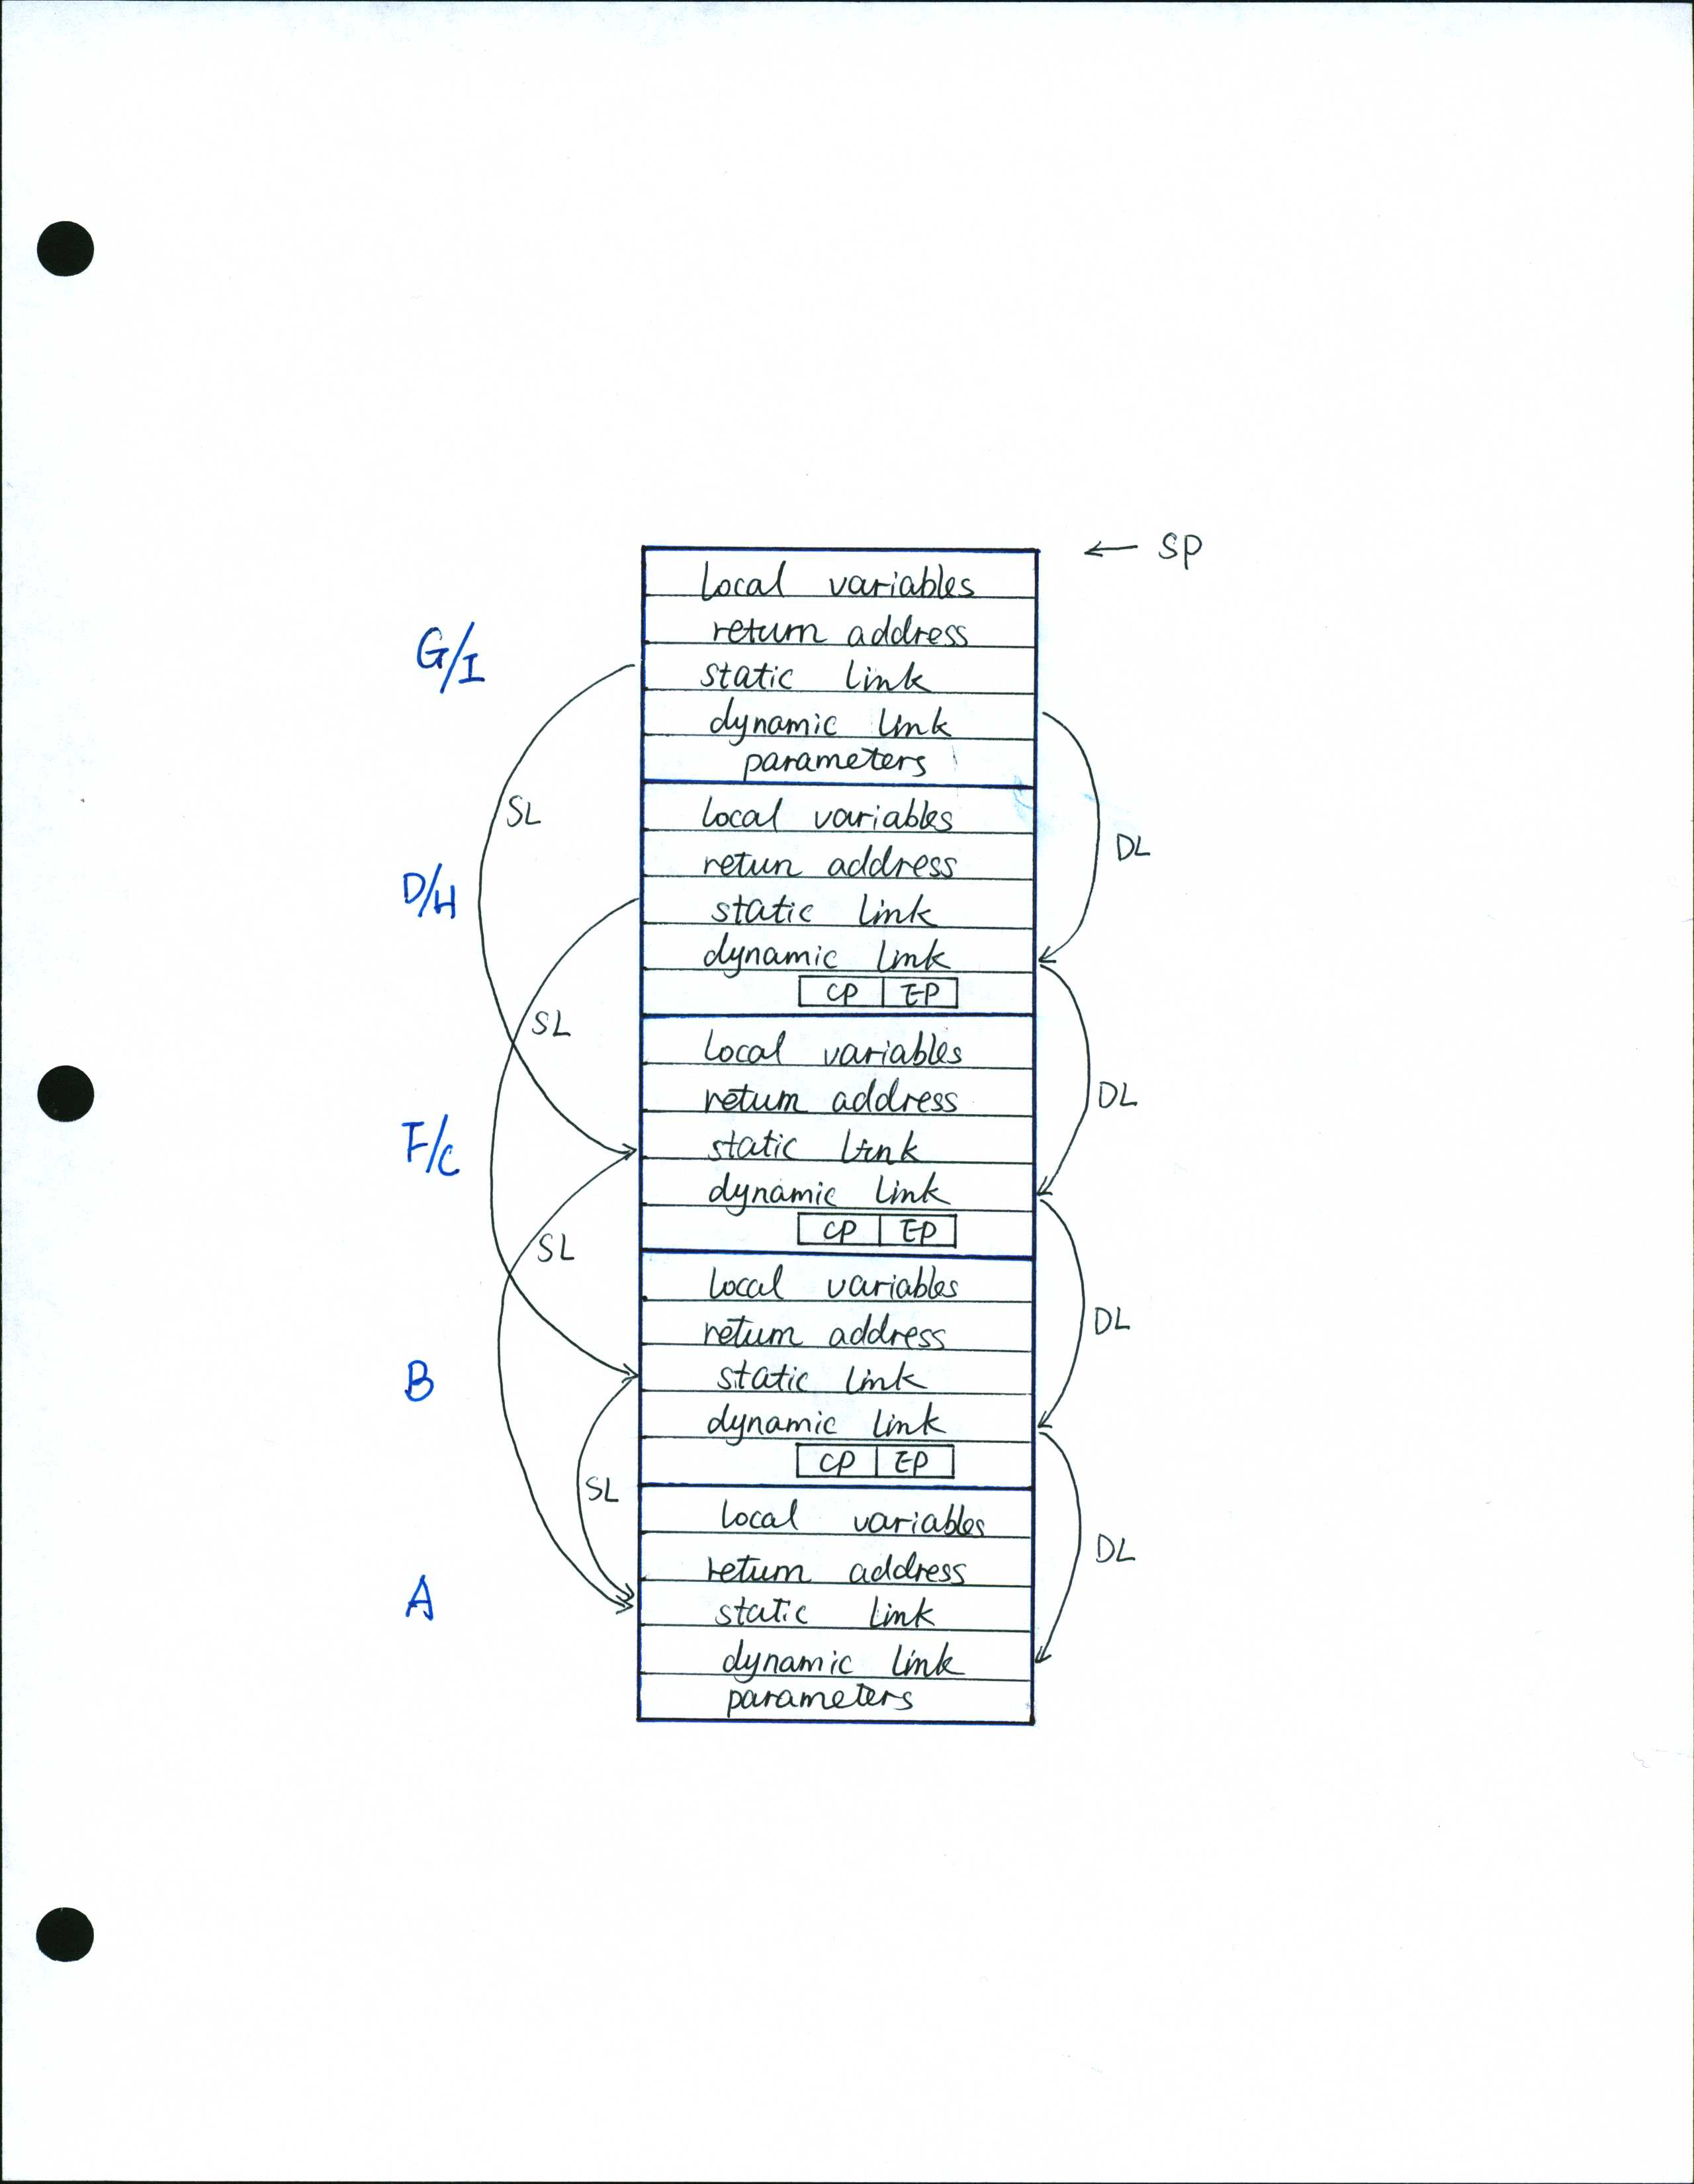
\includegraphics[width=15cm, height=15cm]{stack}
\centering
\end{figure}


\end{document}
